\documentclass[11pt,a4paper]{article}
\usepackage[pdftex,colorlinks,citecolor=blue,urlcolor=blue,linkcolor=red]{hyperref}
\usepackage{amssymb}
\usepackage{amsmath}
\usepackage[dvipsnames]{xcolor}
\usepackage{tikz}
\usetikzlibrary{arrows,decorations.pathmorphing,backgrounds,positioning,fit,petri,patterns}
\usetikzlibrary{decorations.pathreplacing}
\usetikzlibrary{matrix}

\begin{document}

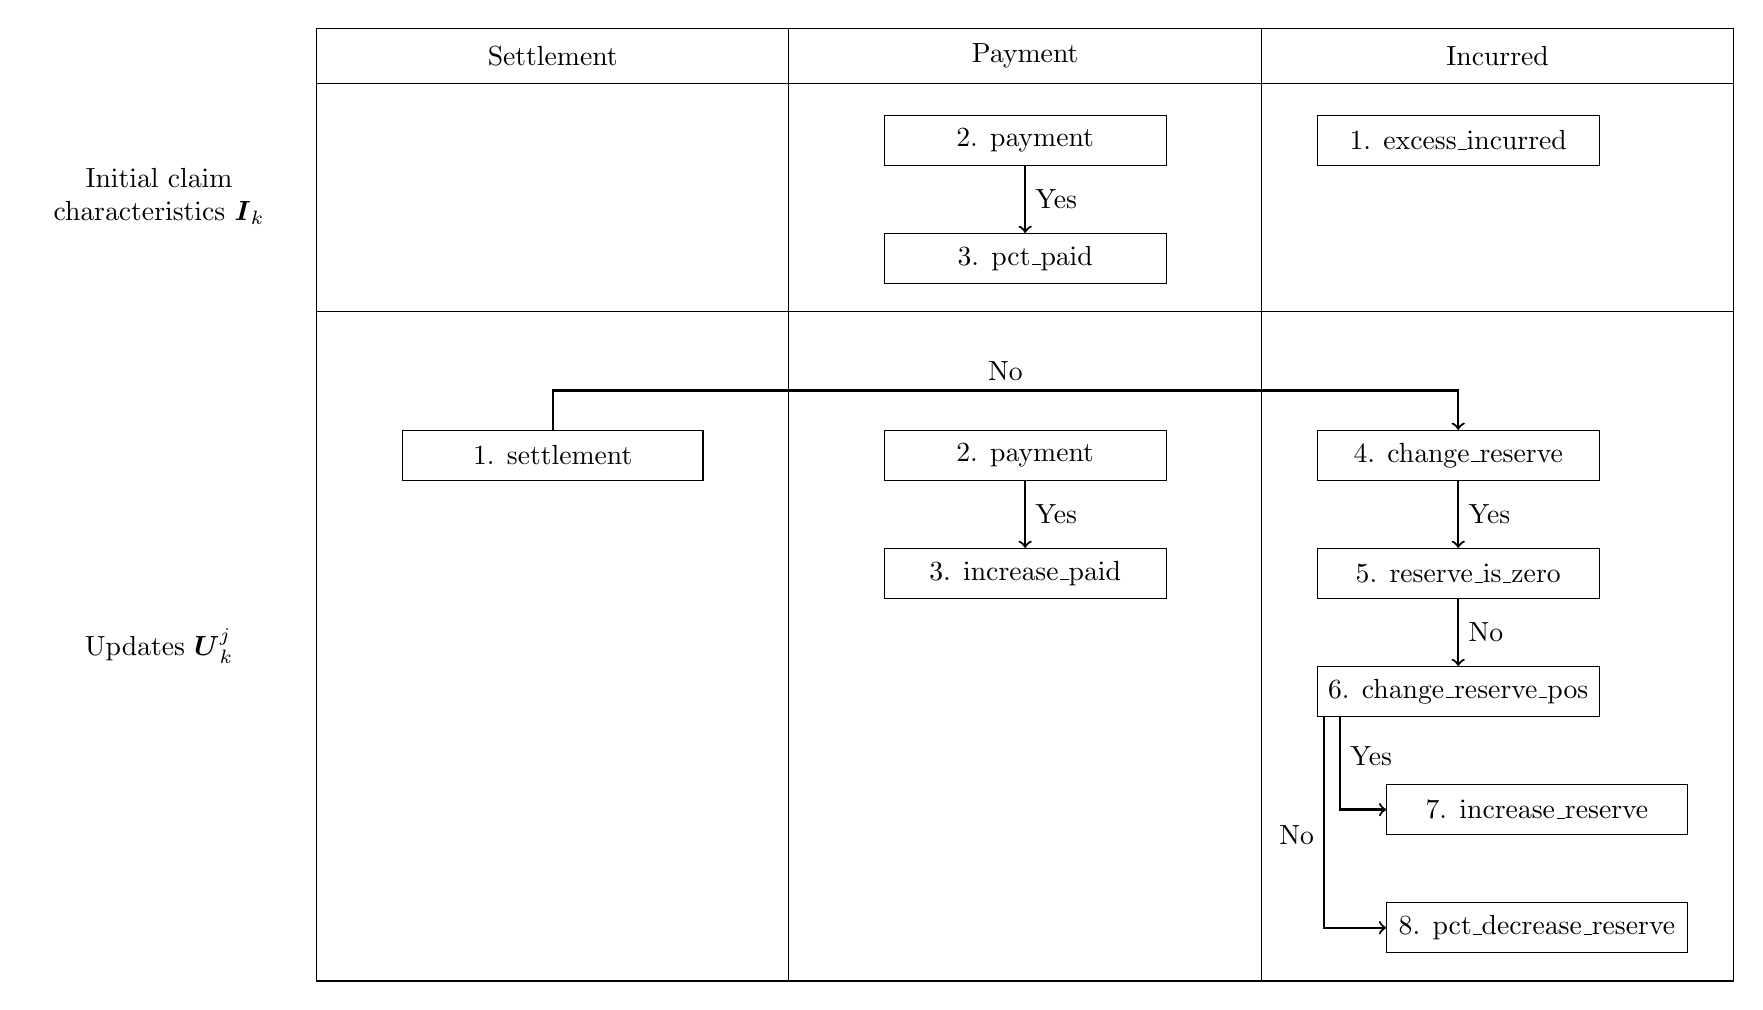
\begin{tikzpicture}
	\tikzset{
  		component/.style = {shape=rectangle, draw, minimum width={width("8. pct\_decrease\_reserve")+2pt}, minimum height={18pt}, anchor = north},
  		box/.style = {shape=rectangle, draw, dashed, minimum width={width("8. pct\_decrease\_reserve")+20pt}, minimum height={95pt}, anchor = north},
  		componentwide/.style = {shape=rectangle, draw, minimum width={width("8. pct\_decrease\_reserve")+2pt}, minimum height={18pt}, anchor = north}
	}
	
	\foreach \x in {0, 6, 12, 18}
	{
		\draw(\x, .6) -- (\x, -11.5);
	}
	
	\foreach \y in {-.1, .6, -3, -11.5}
	{
		\draw(0, \y) -- (18, \y);
	}
	
	\node at (3, .25) {Settlement};		
	\node at (9, .25) {Payment};	
	\node at (15, .25) {Incurred};		
	
	\node[rectangle,fill=white] at (-2, -1.55) {\begin{tabular}{c} Initial claim\\characteristics $\boldsymbol{I}_k$ \end{tabular}};		

	\node[component] (a2) at (9, -.5) {2. payment};
	\node[component] (a3) at (9, -2) {3. pct\_paid};	
	
	\node[component] (a5) at (14.5, -.5) {1. excess\_incurred};		
	
	\draw[->,thick] (a2.south) -- (a3.north) node [midway, right] {Yes};
	
	
	\node[rectangle,fill=white] at (-2, -7.25) {Updates $\boldsymbol{U}_k^j$};			
	
	
	\node[component, minimum width={width("pctwdecreasewreserveaw")+2pt}] (e1) at (3, -4.5) {1. settlement};

	\node[component] (e2) at (9, -4.5) {2. payment};
	\node[component] (e3) at (9, -6) {3. increase\_paid};	

	\node[component] (e4) at (14.5, -4.5) {4. change\_reserve};		
	\node[component] (e5) at (14.5, -6) {5. reserve\_is\_zero};		
	\node[component] (e6) at (14.5, -7.5) {6. change\_reserve\_pos};		
	\node[component, minimum width={width("pctwdecreasewreserveaw")+2pt}] (e7) at (15.5, -9) {7. increase\_reserve};		
	\node[component, minimum width={width("pctwdecreasewreserveaw")+2pt}] (e8) at (15.5, -10.5) {8. pct\_decrease\_reserve};	
	
	\draw[->, thick] (e6.south)++(-1.5,0) -- ++(0, -0.5) node[right]{Yes} |- (e7.west);	
	\draw[->, thick] (e6.south)++(-1.7,0) -- ++(0, -1.5) node[left]{No} |- (e8.west);
	\draw[->, thick] (e2.south) -- (e3.north) node[midway, right] {Yes};
	\draw[->, thick] (e4.south) -- (e5.north) node[midway, right] {Yes};
	\draw[->, thick] (e5.south) -- (e6.north) node[midway, right] {No};
	\draw[->, thick] (e1.north) -- ++(0,0.5) -- ++(11.5, 0) node[midway, above] {No} -| (e4.north)  ;
\end{tikzpicture}

\end{document}